\vspace{5mm}
\section{Comparison of FVM, FEM and DG}

In order to illustrate the different behaviors of FVM, FEM and DG methods, we consider a simple problem with known exact 
solution. The comparison is based on approximately the same number of degrees of freedom (DOF) that was achieved by uniform mesh 
refinements. For compatibility reasons, error is measured in L2 norm. The model problem is the scalar linear advection equation
\be
\label{ade}
\nabla \cdot \beta u\lo x_1, x_2\ro = 0
\ee
in the space-time cylinder $Q_T = \Omega \times \lo 0, T \ro$, where 
$\beta \lo x_1, x_2\ro = (-x_2, x_1) / \left|\bs{x}\right|$ represents a circular counterclockwise 
flow field and $\Omega = [0, 1] \times [0, 1]$. We prescribe the following boundary conditions:
\begin{eqnarray}
u & = & g\ \mbox{on}\ \Gamma_-,\\
g & = & 1\ \mbox{on}\ \Gamma_-^1,\\
g & = & 0\ \mbox{on}\ \Gamma_-^2,
\end{eqnarray}
where $\Gamma_- = \left\{\bs{x} = \lo x_1, x_2\ro\in\partial\Omega:\ \beta\lo x_1, x_2 \ro \cdot \bs{n}(\bs{x}) < 0\right\},\ \Gamma_1 = [0,0.5] \times {0}$, and $\Gamma_-^2 = \Gamma_-\ \backslash\ \Gamma_-^1$. We do not prescribe any boundary condition on the rest of the boundary, i.e. on $\Gamma = \partial\Omega \setminus \Gamma_-$. The exact solution is shown in Fig.~\ref{fig:Exact}.
\begin{figure}[H]
\label{fig:Exact}
\begin{center}
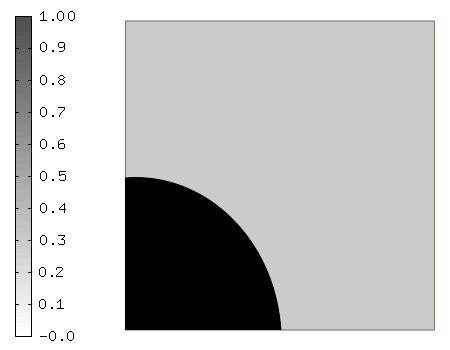
\includegraphics[width=0.48\textwidth]{minor_examples/Exact.png}
\end{center}

\caption{Exact solution.}
\end{figure}
	
\subsection{Finite Volume Method}
We carry out the standard piecewise-constant finite volume discretization of the model problem using the \emph{upwinding} 
numerical flux \cite{compress}. The result corresponding to 32768 DOF is presented in Fig. \ref{fig:fvm000}.
\begin{figure}[H]
\begin{center}
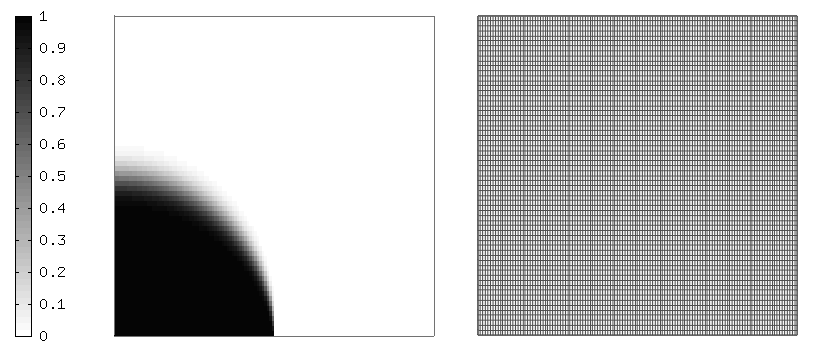
\includegraphics[width=0.9\textwidth]{minor_examples/fvm.png}
\label{fig:fvm000}
\end{center}

\caption{Approximation $u$ (left) and the corresponding mesh (right) with 32768 DIF. Relative L2 error is degrees of 6.19\%.}
\end{figure}
\noindent
We can see that the solution is smeared near the steep gradient although a very fine mesh was used. 
	
\subsection{Finite Element Method}
In order to keep mesh granularity as well as the number of DOF similar to the FVM, we use quadratic elements. For
this demonstration, no stabilization or shock capturing are used. The approximation exhibits the well-known Gibbs 
phenomenon \cite{compress} manifested by spurious oscillations 
in the numerical solution that are visible in Fig. \ref{fig:fem000}.

\begin{figure}[H]
\begin{center}
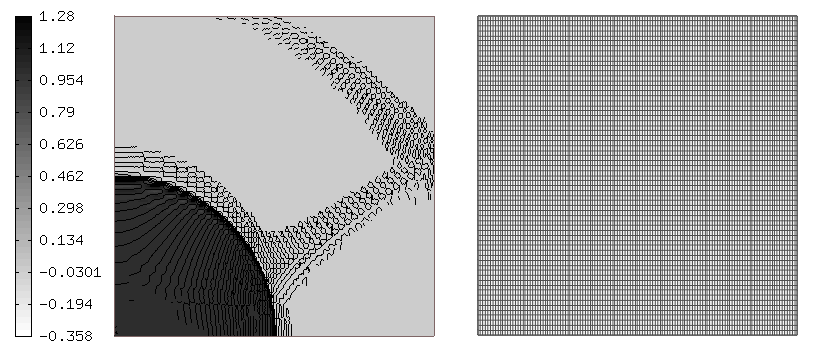
\includegraphics[width=0.9\textwidth]{minor_examples/fem.png}
\caption{Approximation $u$ (left) and the corresponding mesh (right) with polynomial degree $p = 1$ and 33153 DOF. 
Relative L2 error is 7.24\%.}
\label{fig:fem000}
\end{center}
\end{figure}
\noindent
The oscillations can be reduced by employing a suitable stabilization technique such as
Streamline-Upwind Petrov-Galerkin (SUPG) method \cite{SUPG} or others. No such method was applied here. A common disadvantage of these 
methods is that they contain heuristic tuning parameters. 

\subsection{Discontinuous Galerkin Method}
\label{sec:DG}
Since the DG discretization is still less frequently used compared to FVM and FEM, let us 
present briefly its derivation for our model problem. 
Let $\mc{T}_h$ be a triangulation of $\Omega$. For each $K\in\mc{T}_h$ we introduce the notation
\begin{eqnarray}
\partial K^- & = & \left\{x\in\partial K;\beta\lo\bs{x}\ro\cdot\bs{n}\lo\bs{x}\ro <0\right\},\\
\partial K^+ & = & \left\{x\in\partial K;\beta\lo\bs{x}\ro\cdot\bs{n}\lo\bs{x}\ro \geq 0\right\}.
\end{eqnarray}
By $H^k\lo\Omega, \mc{T}_h\ro$ we denote the so-called \itshape broken Sobolev space\upshape:
\be
H^k\lo\Omega,\mc{T}_h\ro = \left\{v\in L^2\lo\Omega\ro;\ v|_K\in H^k\lo K\ro \forall K\in \mc{T}_h\right\}.
\ee
For $u\in H^1\lo\Omega,\mc{T}_h\ro$ we set
\be
u_K^+ = \text{trace of } u|_K \text{ on }\partial K
\ee
(i.e. the interior trace of $u$ on $\partial K$). For each edge $E\subset\partial K\backslash\Gamma$ of $K$, there exists $K'\neq K,\ K'\in\mc{T}_h$, adjacent to $E$ from the opposite side than $K$. Then we put
\be
u_K^- = \text{trace of } u|_{K'} \text{ on } E.
\ee
In this way we obtain the exterior trace $u_K^-$ of $u$ on $\partial K\backslash\Gamma$ and define the jump of $u$ on $\partial K\backslash\Gamma$:
\be
[u]_K = u_K^+ - u_K^-.
\ee
Let $u\in H^1\lo\Omega\ro$ be a solution of the problem~\eqref{ade}. Then $u$ satisfies the identity
\be
\int_K \nabla\cdot\lo\beta u\ro\varphi d\bs{x} = 0,\ \ \varphi\in H^1\lo\Omega,\mc{T}_h\ro,\ K\in\mc{T}_h.
\ee
The application of Green's theorem gives
\begin{eqnarray}
\label{upwinding_derivation_ade}
\int_K \nabla\cdot\lo\beta u\ro\varphi d\bs{x} 
& = & \int_{\partial K}\lo\beta u_K^+\ro\cdot\bs{n}\varphi_K^+ dS - \int_K \lo\beta u\ro\cdot\nabla \varphi d\bs{x}\\\nonumber
& = & \int_{\partial K^-}\lo\beta u_K^+\ro\cdot\bs{n}\varphi_K^+ dS + \int_{\partial K^+}\lo\beta u_K^+\ro\cdot\bs{n}\varphi_K^+ dS\\\nonumber
& - & \int_K \lo\beta u\ro\cdot\nabla \varphi d\bs{x},
\end{eqnarray}
where $\bs{n}$ is the unit outer normal to the element boundary $\partial K$. As $u\in H^1\lo\Omega\ro$, we have $u_K^- = u_K^+$. Moreover, $u_K^-|_{\partial K^-\cap\Gamma_-}:=u|_{\partial K^-\cap\Gamma_-} = g$. 
Then we can write
\begin{eqnarray}
\int_K \nabla\cdot\lo\beta u\ro\varphi d\bs{x} & = & \int_{\partial K^-}\lo\beta u_K^-\ro\cdot\bs{n}\varphi_K^+ dS + \int_{\partial K^+}\lo\beta u_K^+\ro\cdot\bs{n}\varphi_K^+ dS\\\nonumber & - & \int_K \lo\beta u\ro\cdot\nabla \varphi d\bs{x}.
\end{eqnarray}
Applying Green's theorem again, we get the identity
\be
\label{DG_identity_ade}
\int_K \nabla\cdot\lo\beta u\ro\varphi d\bs{x} = \int_{\partial K^-}\lo\beta \lo u_K^+ - u_K^-\ro\ro\cdot\bs{n}\varphi_K^+ dS.
\ee
Setting
\begin{eqnarray}
a_K\lo u, \varphi\ro & = & \int_K \nabla\cdot\lo\beta u\ro\varphi d\bs{x} - \int_{\partial K^-\backslash\Gamma}\lo\beta [u]_K\ro\cdot\bs{n}\varphi_K^+ dS\\\nonumber & - & \int_{\partial K^-\cap\Gamma_-}\lo\beta u_K^+\ro\cdot\bs{n}\varphi_K^+ dS,
\end{eqnarray}
\be
L_K\lo\varphi\ro = \int_{\partial K^-\cap\Gamma_-}\lo\beta g\ro\cdot\bs{n}\varphi_K^+ dS,
\ee
we can rewrite the equation~\eqref{DG_identity_ade} as
\be
\label{final_DG_ade}
a_K\lo u, \varphi\ro = L_K\lo\varphi\ro,\ \ \varphi\in H^1\lo K\ro,\ \ K\in\mc{T}_h.
\ee
This identity makes sense also for $u\in H^1\lo\Omega, \mc{T}_h\ro$. In this case, we can note that in~\eqref{upwinding_derivation_ade}, on $\partial K^-$ (= the inlet of $K$ with respect to the velocity $\beta$) we replace the value $u_K^+$ (the interior trace of u) by $u_K^-$. This means that $upwinding$ is used here, because the value of the trace of $u$ on $\partial K^-$ is taken from the side of $\partial K^-$ against the velocity direction.

The approximate solution is a function $u_h$ satisfying the conditions
\begin{enumerate}
\item $u_h\in V_h = V^{p, -1}\lo\Omega,\mc{T}_h\ro:=\left\{\varphi\in L^2\lo\Omega\ro;\varphi|_K\in P^p\lo K\ro\forall K \in \mc{T}_h\right\}$
\item $a_K\lo u_h, \varphi_h\ro = L_K\lo\varphi_h\ro,\ \forall\varphi_h\in V_h,\ \forall K\in\mc{T}_h$.
\end{enumerate}
Here $p$ stands for the polynomial degree. In general, on each element a different polynomial degree can be used. The approximate solution and test functions are piecewise polynomial functions without any continuity requirement on interfaces between neighboring elements. The continuity requirement is replaced here by the jump term 
$$
\int_{\partial K^-\backslash\Gamma}\lo\beta [u]_K\ro\cdot\bs{n}\varphi_K^+ dS.
$$ 
The $hp$-DG discretization of the Euler equations will be presented in Section~\ref{sec:DGEuler}.
In Fig.~\ref{fig:DG_2} we can see that we successfully avoided the smeared layer close to the steep 
gradient as well as the Gibbs phenomenon in the whole domain. What we have to deal here with on 
the other hand are overshoots and undershoots close to the step gradient. Here the issue was not addressed, for the comparison with the other two methods to be fair. 
There are several approaches how to solve this problem, some of which are described in the last chapter with 
numerical experiments, for the case of the Euler equations.

\begin{figure}[H]
\begin{center}
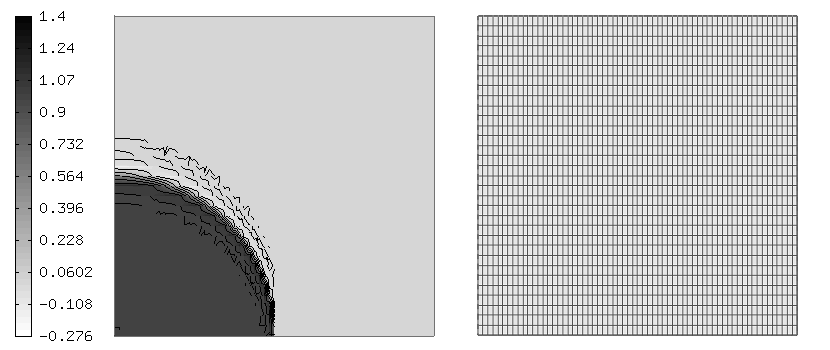
\includegraphics[width=0.9\textwidth]{minor_examples/dg.png}
\caption{Approximation $u$ (left) and the corresponding mesh (right) with polynomial degree $p = 1$ and 32768 DOF. Relative L2 error is 8.89\%.}
\label{fig:DG_2}
\end{center}
\end{figure}
